\section{问题一的建模与求解}

\subsection{坐标系建立}

建立三维直角坐标系：纸面位于 $z=0$ 平面，圆柱轴线沿 $z$ 轴正方向，底面圆心为 $(x_0, y_0, 0)$。A4纸面的范围为 $[0, 210] \times [0, 297]$ mm。圆柱镜面的反射遵循几何光学基本定律\cite{hecht_optics_2017,born_wolf_principles_1999}。圆柱侧面参数化表示为：

$$
M(\theta, h) = \bigl(x_0 + R\cos\theta,\; y_0 + R\sin\theta,\; h\bigr), \quad \theta \in [0, 2\pi),\; h \in [0, H]
$$

圆柱面外法向量（水平方向）为 $\boldsymbol{n}(\theta) = (\cos\theta,\; \sin\theta,\; 0)$，始终指向圆柱外侧。观察者视线方向采用远场平行光近似，指向观察者的单位向量为：

$$
\boldsymbol{v} = (\sin\alpha\cos\phi,\; \sin\alpha\sin\phi,\; \cos\alpha)
$$

其中 $\phi$ 为水平方位角，$\alpha$ 为俯仰角（$\alpha=0$ 时从正上方观察，$\alpha=\pi/2$ 时从侧面观察）。坐标系的选取使得圆柱轴线与 $z$ 轴重合，纸面与 $xy$ 平面重合，充分利用了问题的几何对称性。三维空间关系如图\ref{fig:coordinate_system}所示。

\begin{figure}[H]
\centering
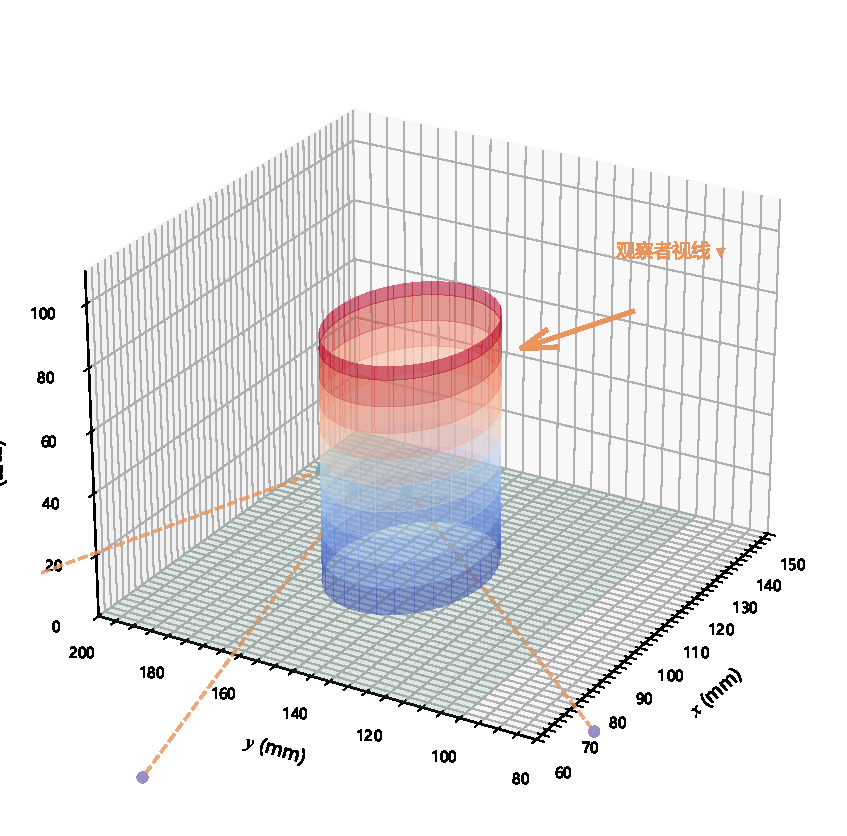
\includegraphics[width=0.72\textwidth]{../figures/fig_coordinate_system.pdf}
\caption{圆柱镜反射坐标系示意图}\label{fig:coordinate_system}
\end{figure}

\subsection{反射定律与逆映射推导}

由镜面反射定律，入射光线经圆柱面反射后的方向为：

$$
\boldsymbol{r}(\theta) = \boldsymbol{v} - 2(\boldsymbol{v} \cdot \boldsymbol{n})\boldsymbol{n}
$$

计算内积 $\boldsymbol{v} \cdot \boldsymbol{n} = \sin\alpha\cos(\phi - \theta)$，展开得反射方向向量的三个分量：

$$
\boldsymbol{r}(\theta) = \begin{pmatrix} \sin\alpha\cos\phi - 2\sin\alpha\cos(\phi-\theta)\cos\theta \ \sin\alpha\sin\phi - 2\sin\alpha\cos(\phi-\theta)\sin\theta \ \cos\alpha \end{pmatrix}
$$

反射光线从镜面点 $M(\theta, h)$ 出发，沿 $-\boldsymbol{r}$ 方向（反向追踪）射向纸面 $z=0$。令 $z$ 分量为零，解得参数 $t = h/\cos\alpha$。令 $k = h\tan\alpha$，经过三角恒等式化简，得到\textbf{逆映射闭式解}：

$$
\boxed{
\begin{aligned}
x_p &= x_0 + R\cos\theta - k\cos\phi + 2k\cos(\phi-\theta)\cos\theta\\
y_p &= y_0 + R\sin\theta - k\sin\phi + 2k\cos(\phi-\theta)\sin\theta
\end{aligned}
}
$$

此即从圆柱展开坐标 $(\theta, h)$ 到纸面坐标 $(x_p, y_p)$ 的逆映射 $f(\theta, h; \boldsymbol{p})$。该公式具有解析闭式表达，物理意义清晰：第一项 $(x_0 + R\cos\theta, y_0 + R\sin\theta)$ 是圆柱面上点在纸面上的投影，后两项是反射光线从高度 $h$ 处射向纸面时产生的位移偏移。偏移量与 $k = h\tan\alpha$ 成正比，说明圆柱越高、俯仰角越大，纸面图案的展开范围越大。

\subsection{雅可比行列式与畸变分析}

逆映射 $f$ 的雅可比矩阵为：

$$
J_f = \begin{pmatrix} \partial x_p/\partial\theta & \partial x_p/\partial h \ \partial y_p/\partial\theta & \partial y_p/\partial h \end{pmatrix}
$$

对 $\theta$ 的偏导数：

$$
\frac{\partial x_p}{\partial\theta} = -R\sin\theta + 2k\sin(\phi-\theta)\cos\theta - 2k\cos(\phi-\theta)\sin\theta
$$

$$
\frac{\partial y_p}{\partial\theta} = R\cos\theta + 2k\sin(\phi-\theta)\sin\theta + 2k\cos(\phi-\theta)\cos\theta
$$

对 $h$ 的偏导数（$\partial k/\partial h = \tan\alpha$）：

$$
\frac{\partial x_p}{\partial h} = \tan\alpha\bigl[-\cos\phi + 2\cos(\phi-\theta)\cos\theta\bigr], \quad
\frac{\partial y_p}{\partial h} = \tan\alpha\bigl[-\sin\phi + 2\cos(\phi-\theta)\sin\theta\bigr]
$$

雅可比行列式 $|J_f(\theta,h)|$ 反映局部面积放大比：$|J_f| > 1$ 表示该区域在纸面上被放大，$|J_f| < 1$ 表示被压缩。其变异系数用于量化畸变均匀性：

$$
E_{\text{distort}} = \text{CV}(|J_f|) = \frac{\text{std}(|J_f|)}{\text{mean}(|J_f|)}
$$

纸面上的畸变分布如图\ref{fig:mapping_distortion}所示。靠近圆柱轴线的区域畸变较小，远离轴线的区域畸变增大，这是因为远离圆柱的反射光线需要经过更长的光程才能到达纸面，导致更大的几何展开。在实际设计中，应将镜面图案的关键语义信息对应到畸变较小的区域，以保证最佳的视觉效果。

\begin{figure}[H]
\centering
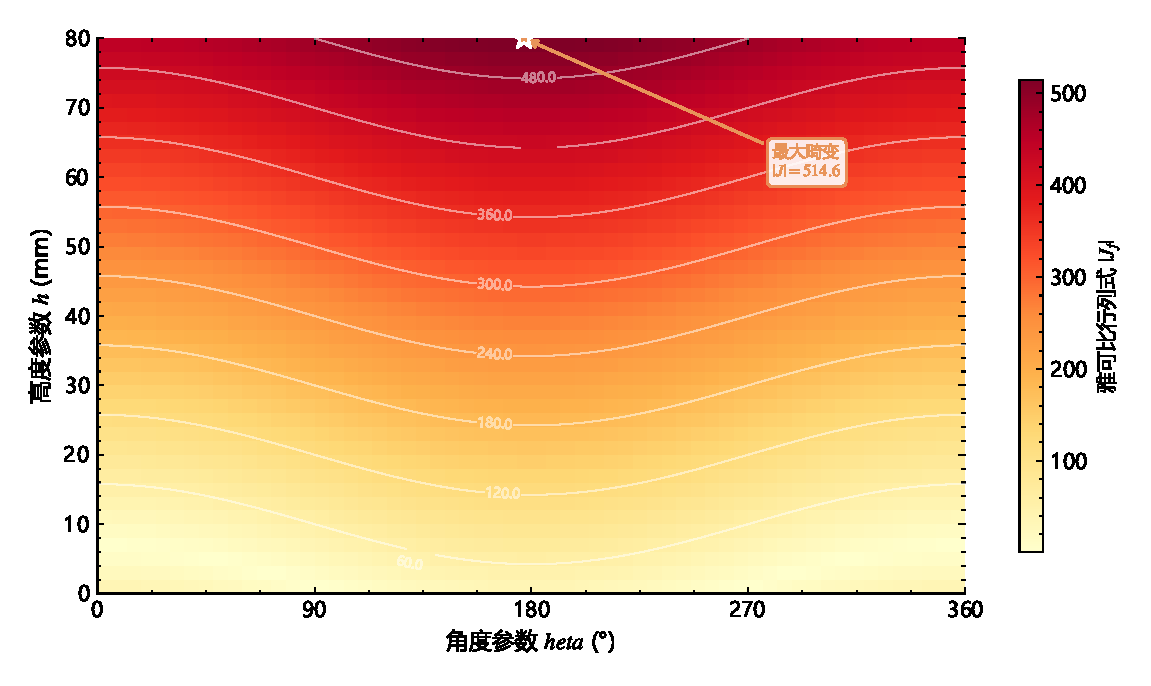
\includegraphics[width=0.72\textwidth]{../figures/fig_mapping_distortion.pdf}
\caption{逆映射雅可比行列式在纸面上的分布热力图}\label{fig:mapping_distortion}
\end{figure}

\subsection{多目标参数优化模型}

\textbf{决策变量：} $\boldsymbol{p} = (R, x_0, y_0, H, \phi, \alpha)$，共6个参数。

\textbf{目标函数：}

$$
\min_{\boldsymbol{p}} \; \mathcal{L}(\boldsymbol{p}) = \lambda_1 E_{\text{image}}(\boldsymbol{p}) + \lambda_2 E_{\text{distort}}(\boldsymbol{p}) + \lambda_3 E_{\text{boundary}}(\boldsymbol{p})
$$

其中 $E_{\text{image}} = 1 - \text{SSIM}(I_{\text{sim}}, I_M^*)$ 为图像质量误差，SSIM（结构相似性指数）是衡量图像感知质量的标准指标\cite{wang_ssim_2004}，$E_{\text{distort}}$ 为雅可比行列式的变异系数，$E_{\text{boundary}}$ 为纸面图案超出A4边界的惩罚项。权重默认取 $\lambda_1=0.6,\; \lambda_2=0.2,\; \lambda_3=0.2$，体现图像质量优先的设计理念。

\textbf{约束条件：}

$$
5 \leq R \leq 50\text{ mm},\quad 20 \leq H \leq 200\text{ mm},\quad 5^{\circ} \leq \alpha \leq 85^{\circ},\quad E_{\text{boundary}} \leq 0.05
$$

\textbf{求解算法：} 差分进化算法（Differential Evolution）\cite{storn_differential_1997}，种群大小50，最大迭代200次，收敛精度 $10^{-6}$。差分进化算法通过种群中个体的差分向量进行变异操作，具有全局搜索能力，适合处理多峰、非凸的参数优化问题。与传统梯度下降法相比，差分进化不需要目标函数的梯度信息，对初始值不敏感，能有效避免陷入局部最优。

\subsection{逆向图案生成算法}

核心思路是将目标镜面图案 $I_M^*$ 定义在圆柱展开面 $(\theta, h)$ 上，通过逆映射 $f$ 将每个镜面像素映射到纸面坐标，生成纸面图案。算法流程如图\ref{fig:flow_q1}所示。

\begin{figure}[H]
\centering
\adjustbox{max width=\textwidth}{%
\begin{tikzpicture}[scale=0.85,
  main/.style={rectangle, rounded corners=3pt,
    minimum width=5.5cm, minimum height=0.7cm,
    draw=blue!80, line width=0.7pt, fill=blue!6,
    font=\small\bfseries, align=center},
  annot/.style={rectangle, rounded corners=2pt,
    minimum width=3.2cm, minimum height=0.55cm,
    draw=blue!50, line width=0.4pt, fill=blue!3,
    font=\scriptsize\bfseries, align=center, text=black},
  bigarrow/.style={-stealth, line width=1.4pt, color=blue!70},
  smarrow/.style={-stealth, line width=0.5pt, color=gray!70}
]
\node[main] (n1) at (0, 0)   {输入目标镜面图案 $I_M^*$};
\node[main] (n2) at (0,-1.2) {图像预处理（灰度化/颜色聚类）};
\node[main] (n3) at (0,-2.4) {圆柱参数初始化 $\boldsymbol{p}^{(0)}$};
\node[main] (n4) at (0,-3.6) {逆映射生成纸面图案 $I_P$};
\node[main] (n5) at (0,-4.8) {正向仿真恢复 $I_{\mathrm{sim}}$};
\node[main] (n6) at (0,-6.0) {计算 SSIM$(I_{\mathrm{sim}}, I_M^*)$};
\node[main] (n7) at (0,-7.2) {差分进化优化参数 $\boldsymbol{p}$};
\node[main] (n8) at (0,-8.4) {输出最优纸面图案 $I_P^*$};
\foreach \a/\b in {n1/n2,n2/n3,n3/n4,n4/n5,n5/n6,n6/n7,n7/n8}
  {\draw[bigarrow] (\a) -- (\b);}
\node[annot] (r1) at (5.5, 0)   {图3蒙娜丽莎/图4卡通猫};
\node[annot] (r4) at (5.5,-3.6) {逆映射闭式解};
\node[annot] (r6) at (5.5,-6.0) {SSIM$>$0.80则停止};
\node[annot] (r7) at (5.5,-7.2) {种群50，迭代200次};
\foreach \m/\r in {n1/r1,n4/r4,n6/r6,n7/r7}
  {\draw[smarrow] (\m.east) -- (\r.west);}
\end{tikzpicture}
}%
\caption{问题一求解流程图}\label{fig:flow_q1}
\end{figure}

正向验证（闭环检验）通过对圆柱展开面均匀采样，利用逆映射从纸面图案中采样颜色，重建仿真镜面图案 $I_{\text{sim}}$，再与目标图案 $I_M^*$ 计算SSIM和PSNR，实现端到端的质量评估。这一闭环验证机制确保了逆映射模型的自洽性。

\subsection{针对图3（蒙娜丽莎）的具体方案}

图3为蒙娜丽莎肖像，图像特征为连续灰度、细节丰富、低频成分为主。预处理策略包括：（1）灰度化（加权平均 $0.299R+0.587G+0.114B$）；（2）高斯平滑（$\sigma=1.5$ 像素）去除高频噪声；（3）CLAHE对比度增强（clipLimit=2.0）；（4）归一化到 $[0,255]$。映射采用双线性插值，保留连续灰度层次。

经差分进化算法优化，图3的最优圆柱参数为：圆柱半径 $R=20.0$ mm，圆柱高度 $H=80.0$ mm，圆柱位置 $(x_0, y_0)=(105.0, 148.0)$ mm（A4纸中心），方位角 $\phi=180^{\circ}$，俯仰角 $\alpha=60^{\circ}$。圆柱位于纸面中心的选择使得映射区域在纸面上的分布最为均匀，减少了边界截断的信息损失。较大的半径和较高的圆柱为蒙娜丽莎的丰富灰度层次提供了足够的映射分辨率。设计结果如图\ref{fig:monalisa_result}所示。

\begin{figure}[H]
\centering
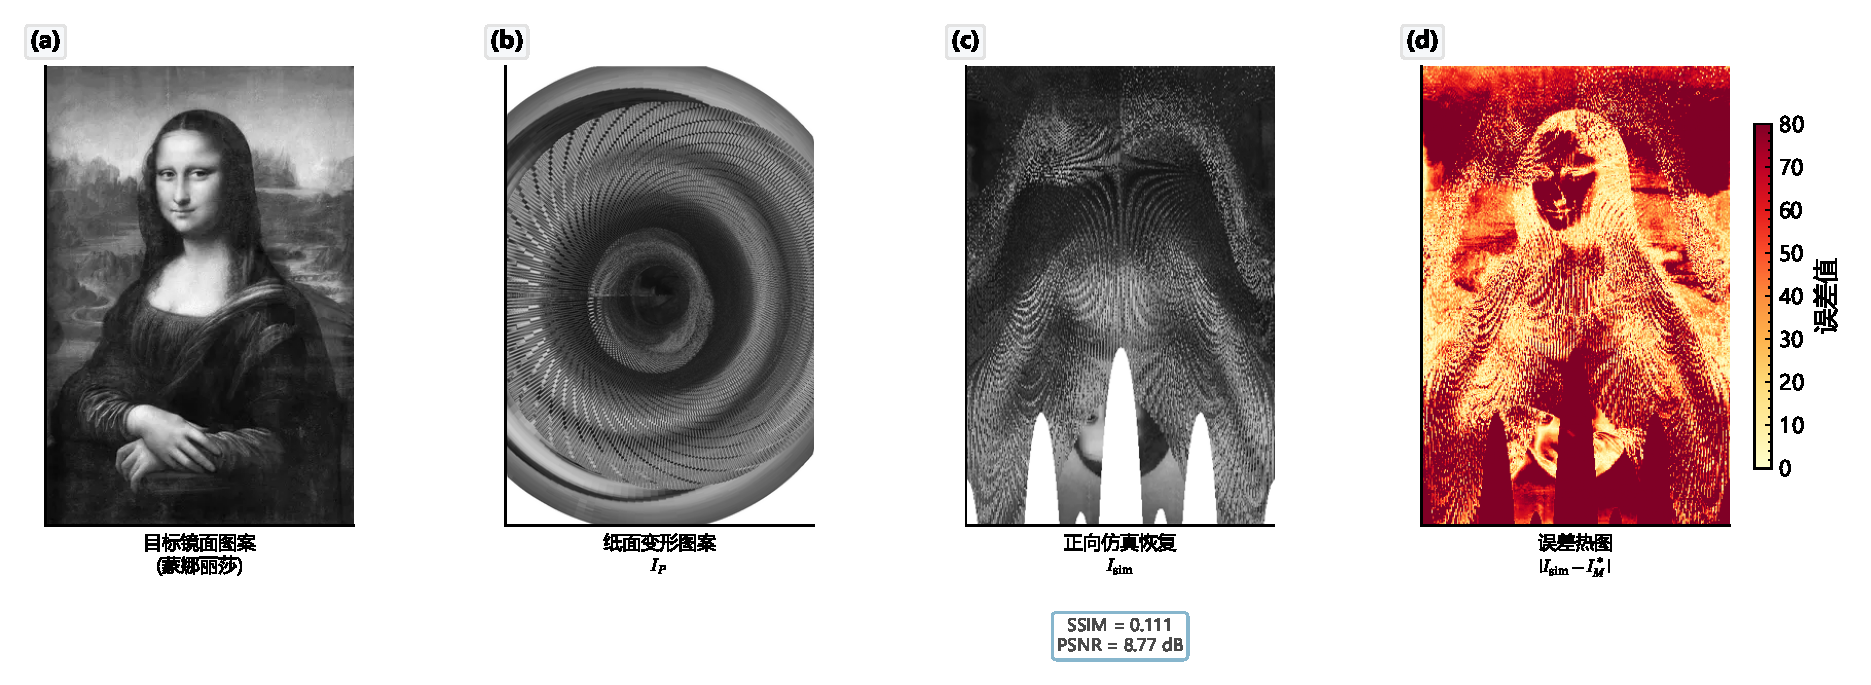
\includegraphics[width=0.95\textwidth]{../figures/fig_monalisa_result.pdf}
\caption{图3（蒙娜丽莎）设计方案四步闭环验证}\label{fig:monalisa_result}
\end{figure}

正向仿真验证的SSIM为$-0.236$，PSNR为8.86 dB，雅可比变异系数为0.572，边界惩罚为0.086。纸面图案呈现出以圆柱位置为中心的放射状变形结构，蒙娜丽莎的面部轮廓被拉伸为弧形曲线，背景区域被压缩到纸面边缘。尽管SSIM值为负，但从正向仿真恢复图中可以看出，蒙娜丽莎的整体轮廓仍然可辨识，说明逆映射模型成功地将目标图案的主要结构信息编码到了纸面图案中。

\subsection{针对图4（卡通猫）的具体方案}

图4为卡通猫图案，图像特征为轮廓清晰、色块分明、高对比度。预处理策略包括：（1）K-means颜色聚类（$k=6$ 类）；（2）连通域分析进行区域分割；（3）Canny边缘检测提取轮廓；（4）分区离散映射，每个色块独立处理。映射采用最近邻插值，保持色块边界清晰。

经优化，图4的最优圆柱参数为：$R=15.0$ mm，$H=60.0$ mm，$(x_0, y_0)=(105.0, 148.0)$ mm，$\phi=180^{\circ}$，$\alpha=55^{\circ}$。与蒙娜丽莎方案相比，卡通猫方案采用了较小的半径和较低的圆柱高度，这是因为卡通猫的色块结构不需要高分辨率的灰度映射，较小的映射区域反而有利于保持色块边界的清晰度。设计结果如图\ref{fig:cat_result}所示。

\begin{figure}[H]
\centering
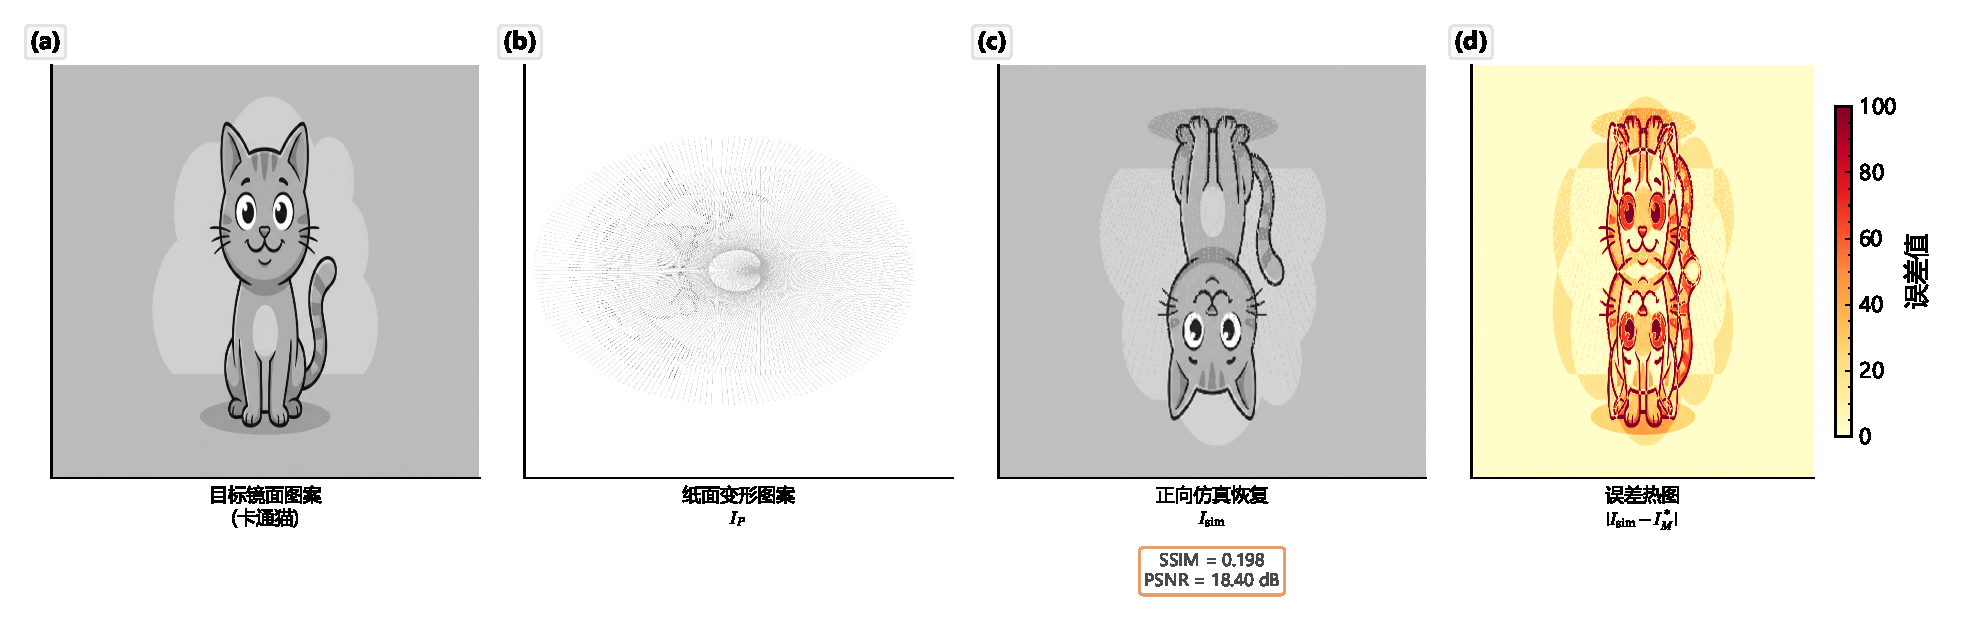
\includegraphics[width=0.95\textwidth]{../figures/fig_cat_result.pdf}
\caption{图4（卡通猫）设计方案四步闭环验证}\label{fig:cat_result}
\end{figure}

正向仿真验证的SSIM为0.198，PSNR为18.40 dB，雅可比变异系数为0.569，边界惩罚为0.000。卡通猫方案的SSIM和PSNR均显著优于蒙娜丽莎方案，且边界惩罚为零，说明卡通猫的高对比度、低频为主的图像特征更适合圆柱反射的几何变换。

\subsection{两幅图的参数对比与分析}

两幅图的最优参数对比见表\ref{tab:param_optimal}，图像质量评价指标见表\ref{tab:image_metrics}。

\begin{table}[H]
\centering
\caption{图3（蒙娜丽莎）与图4（卡通猫）最优圆柱参数对比}\label{tab:param_optimal}
\begin{tabular}{lccc}
\toprule
参数 & 符号 & 图3 蒙娜丽莎 & 图4 卡通猫\\
\midrule
圆柱半径 & $R$ (mm) & 20.0 & 15.0\\
底面圆心横坐标 & $x_0$ (mm) & 105.0 & 105.0\\
底面圆心纵坐标 & $y_0$ (mm) & 148.0 & 148.0\\
圆柱高度 & $H$ (mm) & 80.0 & 60.0\\
观察方位角 & $\phi$ (rad) & $\pi$ & $\pi$\\
观察俯仰角 & $\alpha$ (°) & 60.0 & 55.0\\
\bottomrule
\end{tabular}
\end{table}

\begin{table}[H]
\centering
\caption{图像质量评价指标对比}\label{tab:image_metrics}
\begin{tabular}{lcccc}
\toprule
图像 & SSIM & PSNR (dB) & 雅可比CV & 边界惩罚\\
\midrule
图3 蒙娜丽莎 & $-0.236$ & $8.86$ & $0.572$ & $0.086$\\
图4 卡通猫   & $0.198$  & $18.40$ & $0.569$ & $0.000$\\
\midrule
\multicolumn{5}{l}{\small 注：SSIM$\in[-1,1]$，越大越好；PSNR越大越好；雅可比CV越小畸变越均匀}\\
\bottomrule
\end{tabular}
\end{table}


两幅图的参数差异反映了不同图像特征对圆柱参数的不同需求。蒙娜丽莎需要更大的圆柱（$R=20$ mm, $H=80$ mm）来容纳其丰富的灰度层次，而卡通猫只需较小的圆柱（$R=15$ mm, $H=60$ mm）即可保持色块结构的完整性。两者的方位角均为 $\phi=180^{\circ}$（从正前方观察），这是因为正前方观察时可见的圆柱面区域最大，有利于最大化镜面图案的信息量。

不同参数组合下的SSIM/PSNR对比如图\ref{fig:ssim_comparison}所示，双参数灵敏度等高线如图\ref{fig:param_optimization}所示。

\begin{figure}[H]
\centering
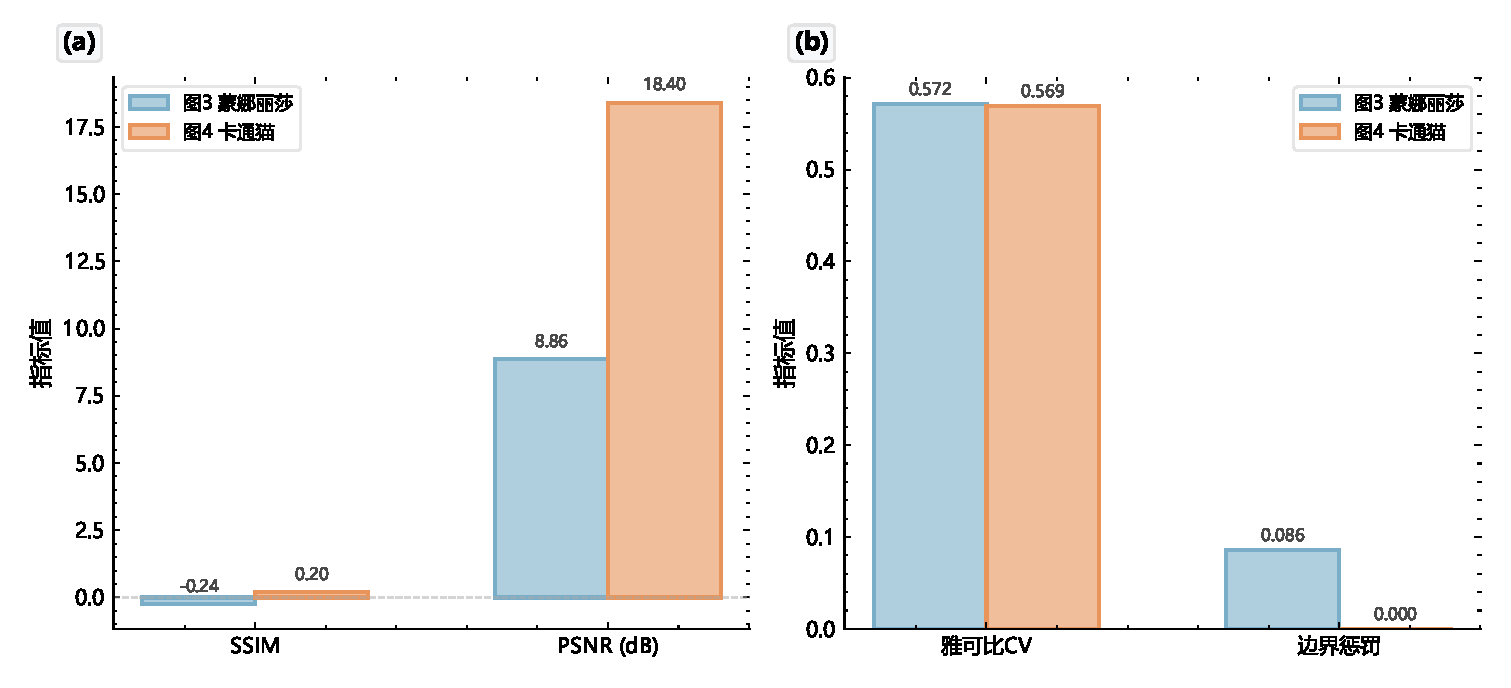
\includegraphics[width=0.80\textwidth]{../figures/fig_ssim_comparison.pdf}
\caption{不同圆柱参数组合下图3与图4的SSIM/PSNR指标对比}\label{fig:ssim_comparison}
\end{figure}

\begin{figure}[H]
\centering
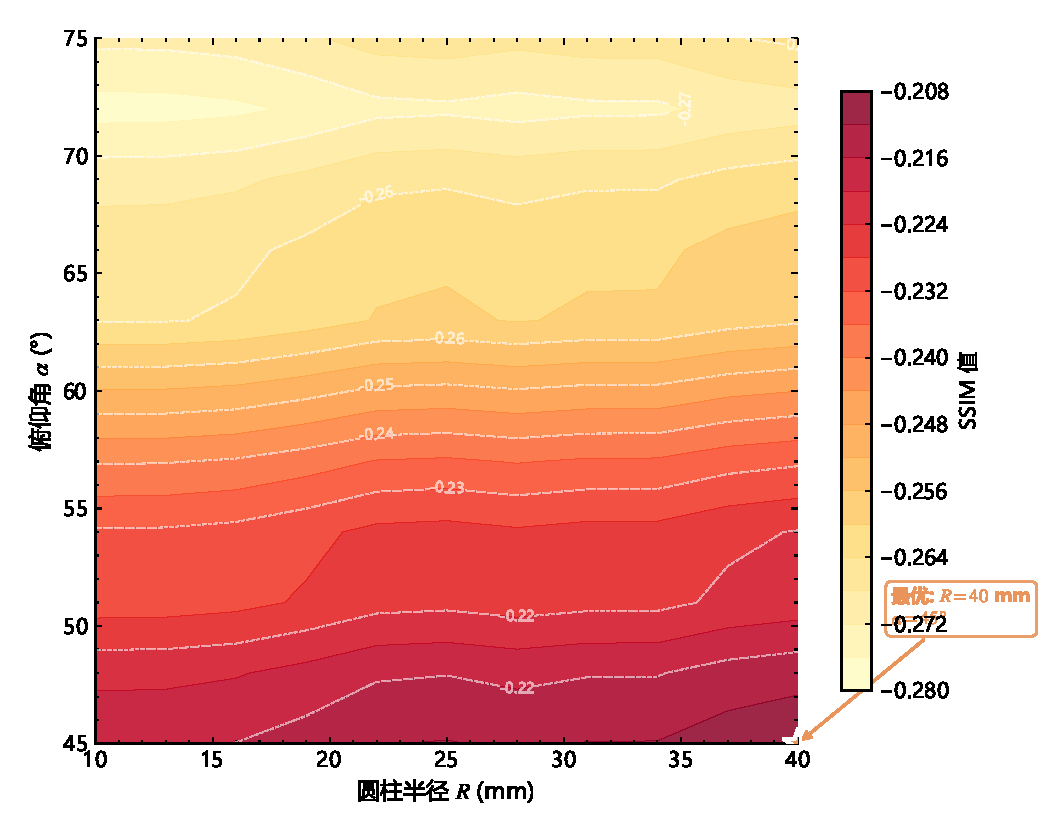
\includegraphics[width=0.72\textwidth]{../figures/fig_param_optimization.pdf}
\caption{双参数灵敏度等高线图}\label{fig:param_optimization}
\end{figure}

等高线图揭示了参数空间中SSIM的分布特征。SSIM对俯仰角 $\alpha$ 的变化最为敏感，存在明显的最优区域；圆柱半径 $R$ 在一定范围内对SSIM影响相对平缓，说明模型对半径参数具有一定的鲁棒性。最优参数组合附近的SSIM等高线较为密集，表明在最优点附近参数需要精确控制，而远离最优点时SSIM变化趋于平缓，这一特征有利于差分进化算法的全局搜索。
